\subsection{Anonymity-oriented Edge Perturbing}
\begin{figure}
    \captionsetup{justification=centering,margin=1cm}
       \begin{subfigure}[b]{0.45\textwidth}
        \centering
        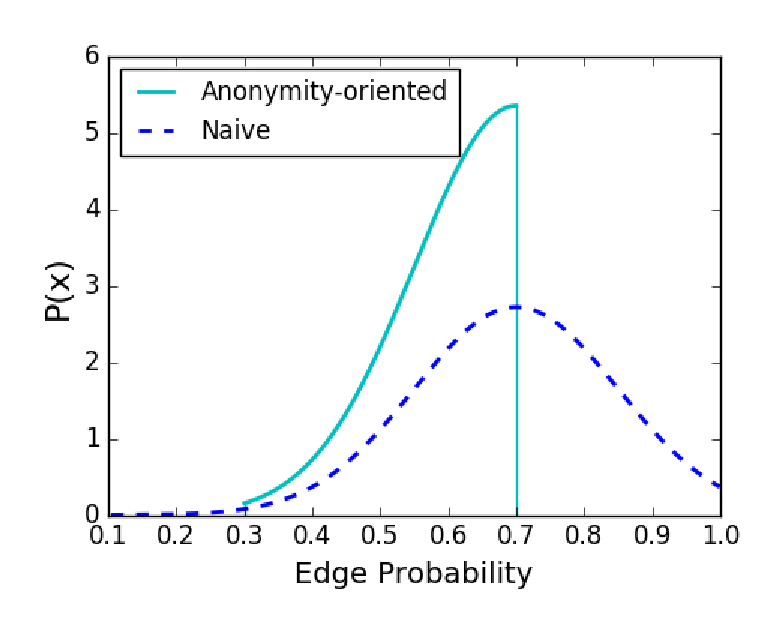
\includegraphics[scale=0.35]{figures/DegreeAUG/AnonymityEP.eps}
        \caption{\small{Anonymity-oriented Edge Perturbing}}
        \label{fig:anonymityEP}
    \end{subfigure}%
    \centering
        \begin{subfigure}[b]{0.45\textwidth}
            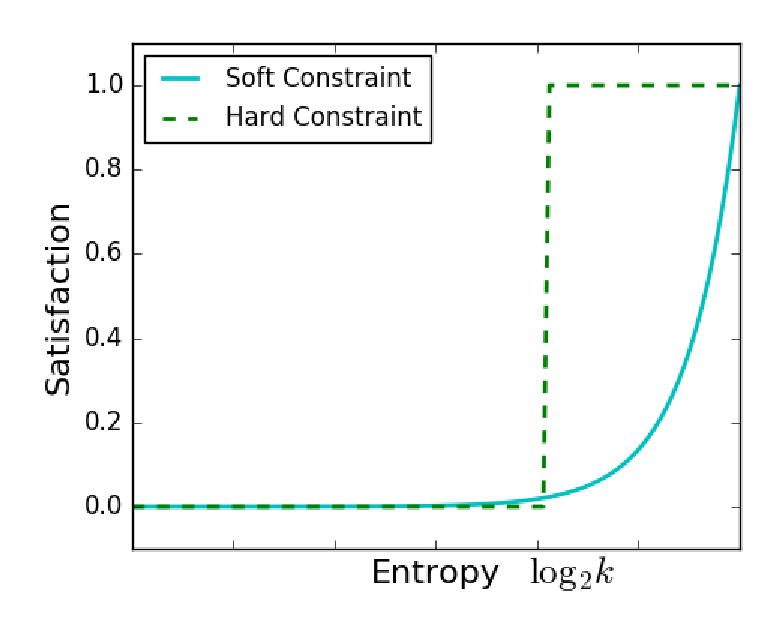
\includegraphics[scale=0.35]{figures/DegreeAUG/constraint.eps}
            \caption{\small{Relaxing $k$-obfuscation constraint}}
            \label{fig:constraintRelax}
        \end{subfigure} 
\end{figure}
As ever discussed, the existing uncertainty injecting scheme is designed for deterministic graphs and can not be used to handle uncertain graphs directly. Given the uncertainty level $\sigma(e)$, a natural strategy is to consider the partial edge addition and deletion in a random way as shown in Figure \ref{fig:anonymityEP}. Through the analysis of the impact of a single edge probability alteration, we give a anonymity-oriented perturbing heuristics which is able to constraint the potential range of edge prob perturbing (referred to C). For each selected edge $e \in E_{c}$ and the assigned uncertainty level $\sigma(e)$, we alter its existence probability as 
\vj
\begin{equation*}
    \tilde{\mathit{p}}(e):=\mathit{p}(e) + (1-2 \mathit{p}(e)) \cdot r_{e} 
    \svj
\end{equation*} 
Where the random perturbation $r_{e}$ is generated according to $\sigma(e)$ as Eq. \ref{eq:gen}. Namely, for an edge with the probability $p$, we only consider potential edge probability $\tilde{p}$ in the limited range that more likely contributes to higher graph anonymity. Clearly, previous scheme defined in deterministic graph becomes a special case of our approach. We proceed to elaborate the rationality and the benefit of this anonymity-oriented edge perturbing scheme by treating it as a constraint satisfaction problem. 
  
\subsubsection{Basics}
Let us consider $k$-obfuscate a given node $v$ as a single constraint $c_{v}$ for the target anonymization graph. Then, according to the definition \ref{obfCon}, the satisfaction of the constraint $c_{v}$ is defined as
\begin{equation*}
    \mathtt{c}_{v}:=
        \begin{cases}
                1  & H(Y_{P(v)}) \geq \log_{2}{k} \\
                0  & otherwise \\
         \end{cases}
\end{equation*}
Namely, given the considered degree-based re-identification scenario, we lower bound the entropy of degree distribution over the anonymized graph by $log_{2}{k}$. Accordingly, whether the anonymized graph $k$-obfuscates all the nodes can be expressed as degree of joint satisfaction.
\vj
\begin{align*}
    \mathcal{C(\mathcal{G})} &= \prod_{v \in V} \mathtt{c}_{v} \\
                &=\prod_{\omega} \underbrace{\mathtt{c} \ldots \mathtt{c}}_{s(\omega)}
    \svj
\end{align*}
The uncertain graph is said to $k$-obfuscate all the nodes if and only if the $C(\mathcal{G})$ equals 1.  
\subsubsection{Re-visiting graph anonymity}
As shown in Figure \ref{fig:constraintRelax}, the original satisfaction function is not everywhere differentiable.To simply the anonymity analysis, we approximate the individual constraint $c_{v}$ to a fuzzy relation in which the satisfaction degree of a constraint is defined as a continuous and differentiable function, going from fully violated to fully satisfied. A natural candidate for soft satisfaction function is,
\svj  
\begin{equation*}
    C_{v} = e^{H(Y_{P(v)})-\log_{2}{|V|}}
    \svj
\end{equation*}
According to this approximation, the satisfaction function of $k$-obfuscate all the nodes can be rewritten as
\svj
\begin{equation*}
   \mathcal{C}(\mathcal{G}) \propto \prod_{\omega} \underbrace{e^{H(Y(\omega)} \ldots e^{H(Y(\omega))}}_{s(\omega)}
\end{equation*}
While the original satisfaction is a binary value, the approximated satisfaction value lies in the continuous range $[0,1]$. Note that, the higher satisfaction score indicates the higher level of anonymity achieved. Taking logarithm for both side, we get the concise formula as 
\svj
\begin{equation*}
    \log \mathcal{C}(\mathcal{G})=\sum_{\omega} s(\omega) \cdot H(Y(\omega)
\end{equation*}
Regarding the property $P$, it equals the weighted sum of entropy over all possible values $\omega$, where $s(\omega)$ is the expected number of vertices with property value $\omega$ over all possible worlds. Targeting at high anonymity, we wish to increase the weighted sum of entropy. 

\subsubsection{Greedy search of graph anonymity}
% \begin{figure}
%     \centering
%     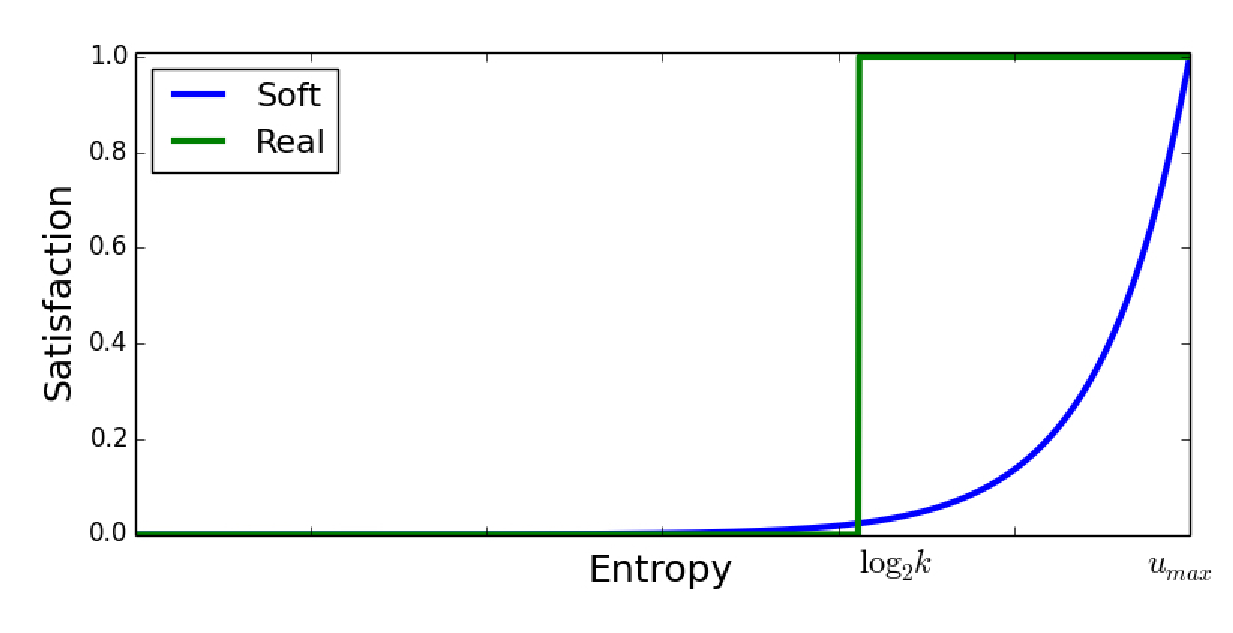
\includegraphics[scale=0.3]{figures/fuzzyConstraint.eps}
%     \caption{Relaxing Constraint}
%     \label{fig:rc}
% \end{figure}
The remaining issue is to connect the single edge probability alteration with the objective. With respects to node degree, a graph can be represented as one matrix as shown in figure \ref{fig:constraintRelax}. The weighted sum of entropy is related with graph coding. Here, we utilize entropy encoding, especially Huffman coding. From the coding perspective, we have two different angles to perform graph coding: row or column of degree matrix. The encoded length should be equal to each other, as shown in the following equation.  
\svj
\begin{equation*}
    \sum_{v} H(v) + n \log{n} = \sum_{\omega} s(\omega) \cdot H(Y(\omega))+ H(s(\omega))
    \svj
    \label{wegithedEn}
\end{equation*}
It indicates that higher global anonymity of a uncertain graph can be achieved by increasing the entropy of individual nodes when the global distribution $H(\omega)$ keeps constant. 

Note that, the probability change over a specific edge only affects degree distributions of its connected nodes. 
To further simply the problem, we assume that the impact of edge perturbing is independent to each other. Recall that, we suggest implementing perturbation to less anonymized nodes. In the case of degree obfuscation, they are nodes with high degree. For a node $v$ with high degree, the probability distribution of its degree $d_{v}$ may be approximated as the normal distribution as implied by the Central Limit Theorem. Hence, its induced entropy $H(v)$ can be approximated as $\frac{1}{2} {\ln (2 \pi e \sigma^2)}$. 

Targeting at maximizing the graph anonymity, we take steps proportion to the positive gradient with respect to the choice of individual edge probabilities. 
\svj
\begin{equation*}
    \frac{\partial \sum_{\omega} s(\omega) H(Y(\omega))} {\partial p(e)} \propto (1-2\mathit{p}(e))  
\end{equation*} 
Therefore, 
\vj
\begin{equation*}
    \tilde{\mathit{p}}(e):=\mathit{p}(e) + (1-2 \mathit{p}(e)) \cdot r_{e}
\end{equation*} 
Namely, our approach simulates one iteration of batch gradient ascent method for finding the local maximum of weighted entropy sum or the anonymity level. 